\section{Una puerta}

\subsubsection{Puerta ancha (3,6 m)}

\begin{figure}[H]
    \centering
    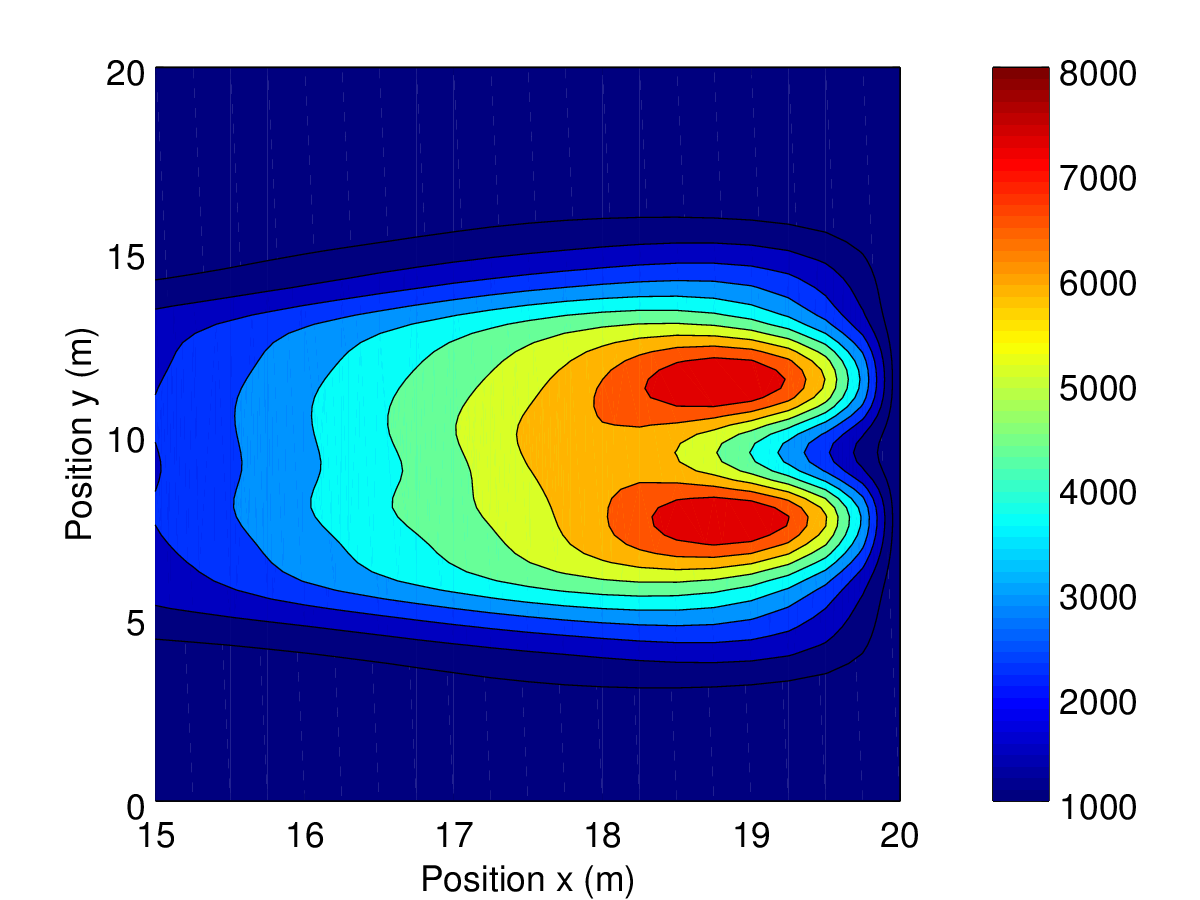
\includegraphics[height=5.5cm]{figuras/press_225p_v4_onedoor_3_6.png}
    \caption[width=5cm]{Isobaras cercanas a la puerta; la escala a la derecha está expresada en [PV]=N.m. La salida está centrada en la posición $x=20$~m e $y=10$~m y tiene ancho $L=3,6$~m. El recinto es de $20\times 20$~(m) con 225 individuos. La gráfica corresponde a valores medios a lo largo de 30 procesos de evacuación. Se usó un grillado de 1m$^2$ para promediar el campo de presiones (PV). La velocidad deseada de los individuos fue de $v_d=4$~m/s.}
    \label{isobaras_3_6m}
\end{figure}

\begin{figure}[H]
    \centering
    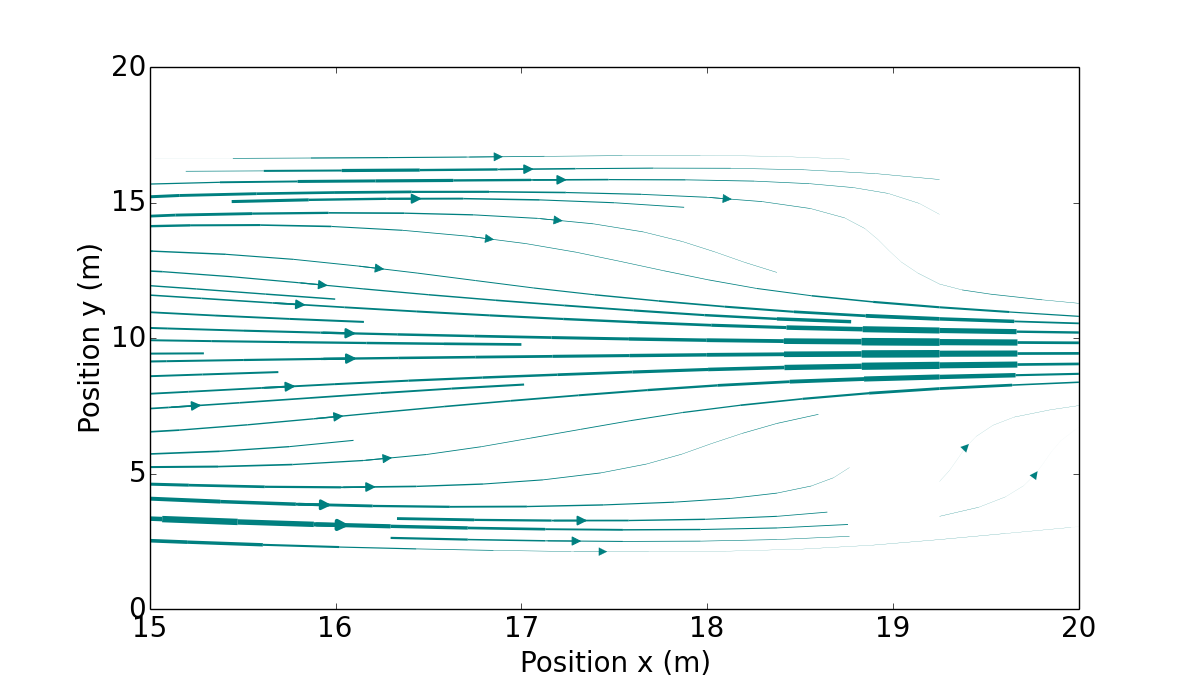
\includegraphics[height=5.5cm]{figuras/flujo_door_3_6m.png}
    \caption[width=5cm]{Gráfico de velocidad. La salida está centrada en la posición $x=20$~m e $y=10$~m y tiene ancho $L=3,6$~m. El recinto es de $20\times 20$~(m) con 225 individuos. La gráfica corresponde a valores medios a lo largo de 30 procesos de evacuación. Se usó un grillado de 1m$^2$ para promediar el campo de velocidades. La velocidad deseada de los individuos fue de $v_d=4$~m/s.}
    \label{sintesis}
\end{figure}

\begin{figure}[H]
    \centering
    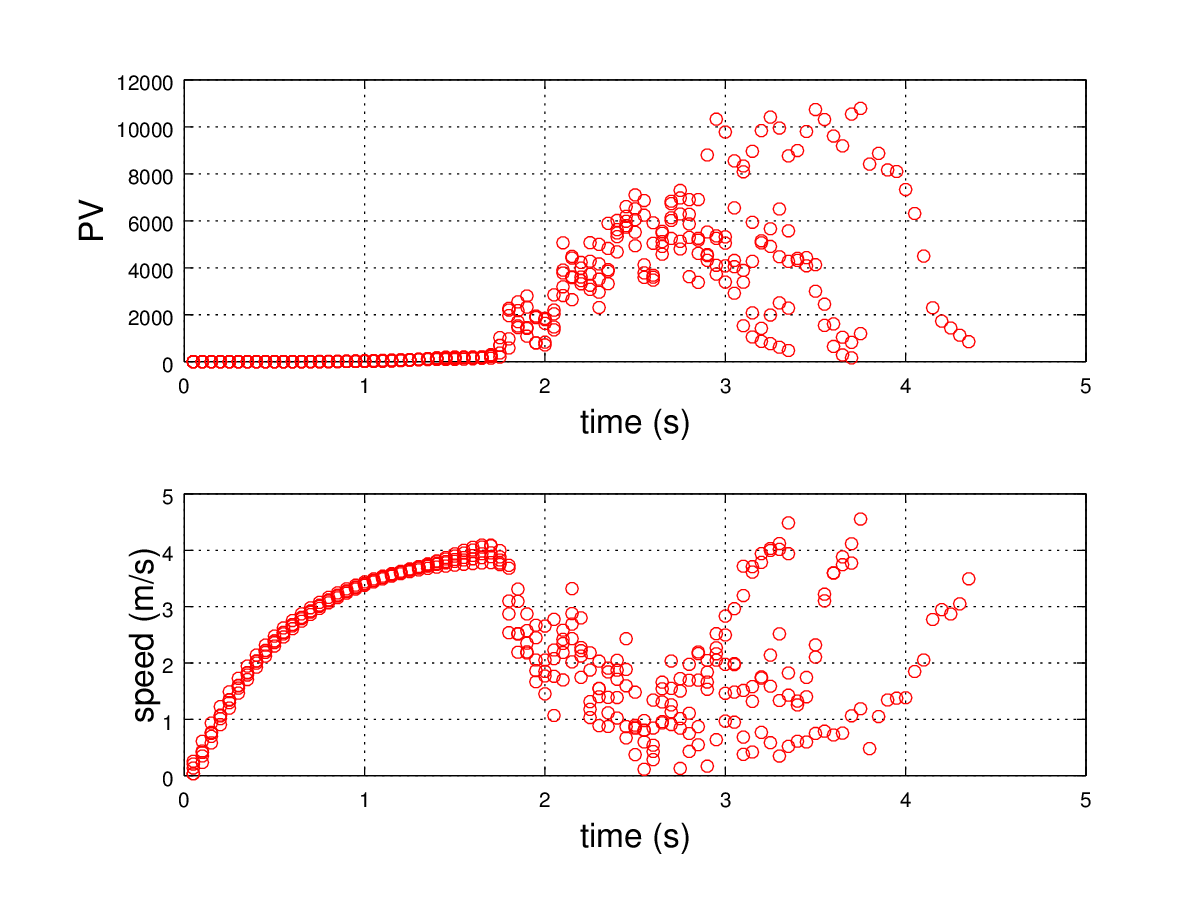
\includegraphics[height=5.5cm]{figuras/pv_vel_t_100_3_6.png}
    \caption[width=5cm]{Gráfico de velocidad(inferior) y presión(superior) en función del tiempo para un individuo ubicado inicialmente en $x=10$~m e $y=10$~m.  La salida está centrada en la posición $x=20$~m e $y=10$~m y tiene ancho $L=3,6$~m. El recinto es de $20\times 20$~(m) con 225 individuos. La gráfica corresponde a cinco iteraciones diferentes (variando la velocidad incial). La velocidad deseada del individuo fue de $v_d=4$~m/s.}
    \label{sintesis}
\end{figure}

\subsubsection{Puerta angosta (1,2 m)}

\begin{figure}[H]
    \centering
    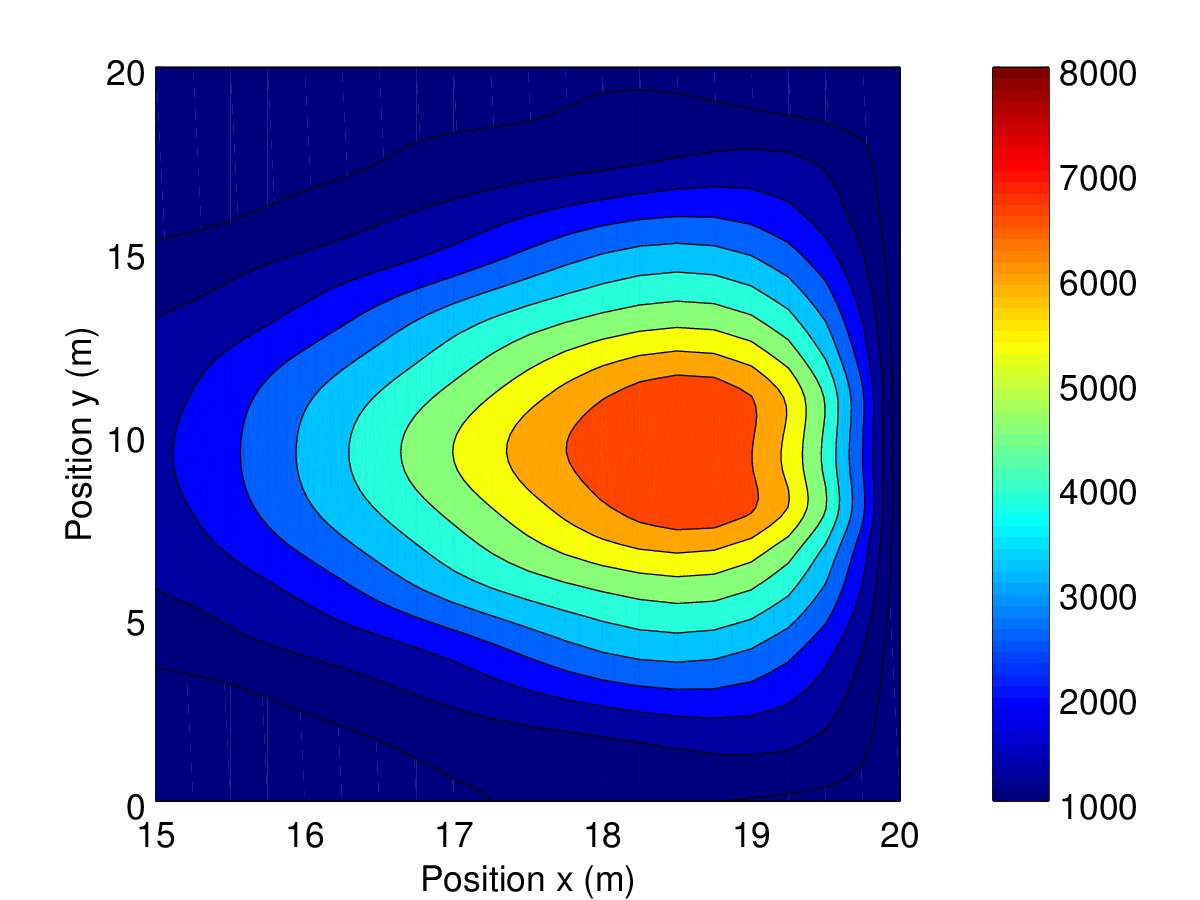
\includegraphics[height=5.5cm]{figuras/press_225p_v4_onedoor_1_2.png}
    \caption[width=5cm]{Isobaras cercanas a la puerta; la escala a la derecha está expresada en [PV]=N.m. La salida está centrada en la posición $x=20$~m e $y=10$~m y tiene ancho $L=1,2$~m. El recinto es de $20\times 20$~(m) con 225 individuos. La gráfica corresponde a valores medios a lo largo de 30 procesos de evacuación. Se usó un grillado de 1m$^2$ para promediar el campo de presiones (PV). La velocidad deseada de los individuos fue de $v_d=4$~m/s.}
    \label{isobaras_1_2m}
\end{figure}

\begin{figure}[H]
    \centering
    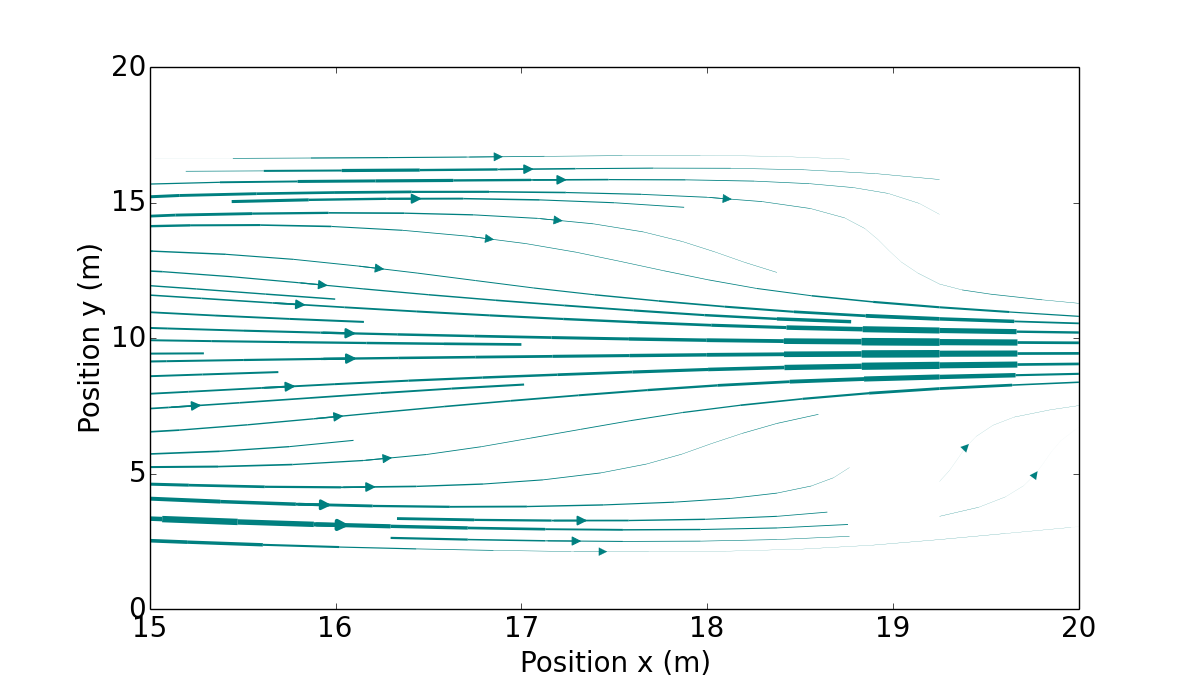
\includegraphics[height=5.5cm]{figuras/flujo_door_1_2m.png}
    \caption[width=5cm]{Gráfico de velocidad. La salida está centrada en la posición $x=20$~m e $y=10$~m y tiene ancho $L=1,2$~m. El recinto es de $20\times 20$~(m) con 225 individuos. La gráfica corresponde a valores medios a lo largo de 30 procesos de evacuación. Se usó un grillado de 1m$^2$ para promediar el campo de velocidades. La velocidad deseada de los individuos fue de $v_d=4$~m/s.}
    \label{sintesis}
\end{figure}

\begin{figure}[H]
    \centering
    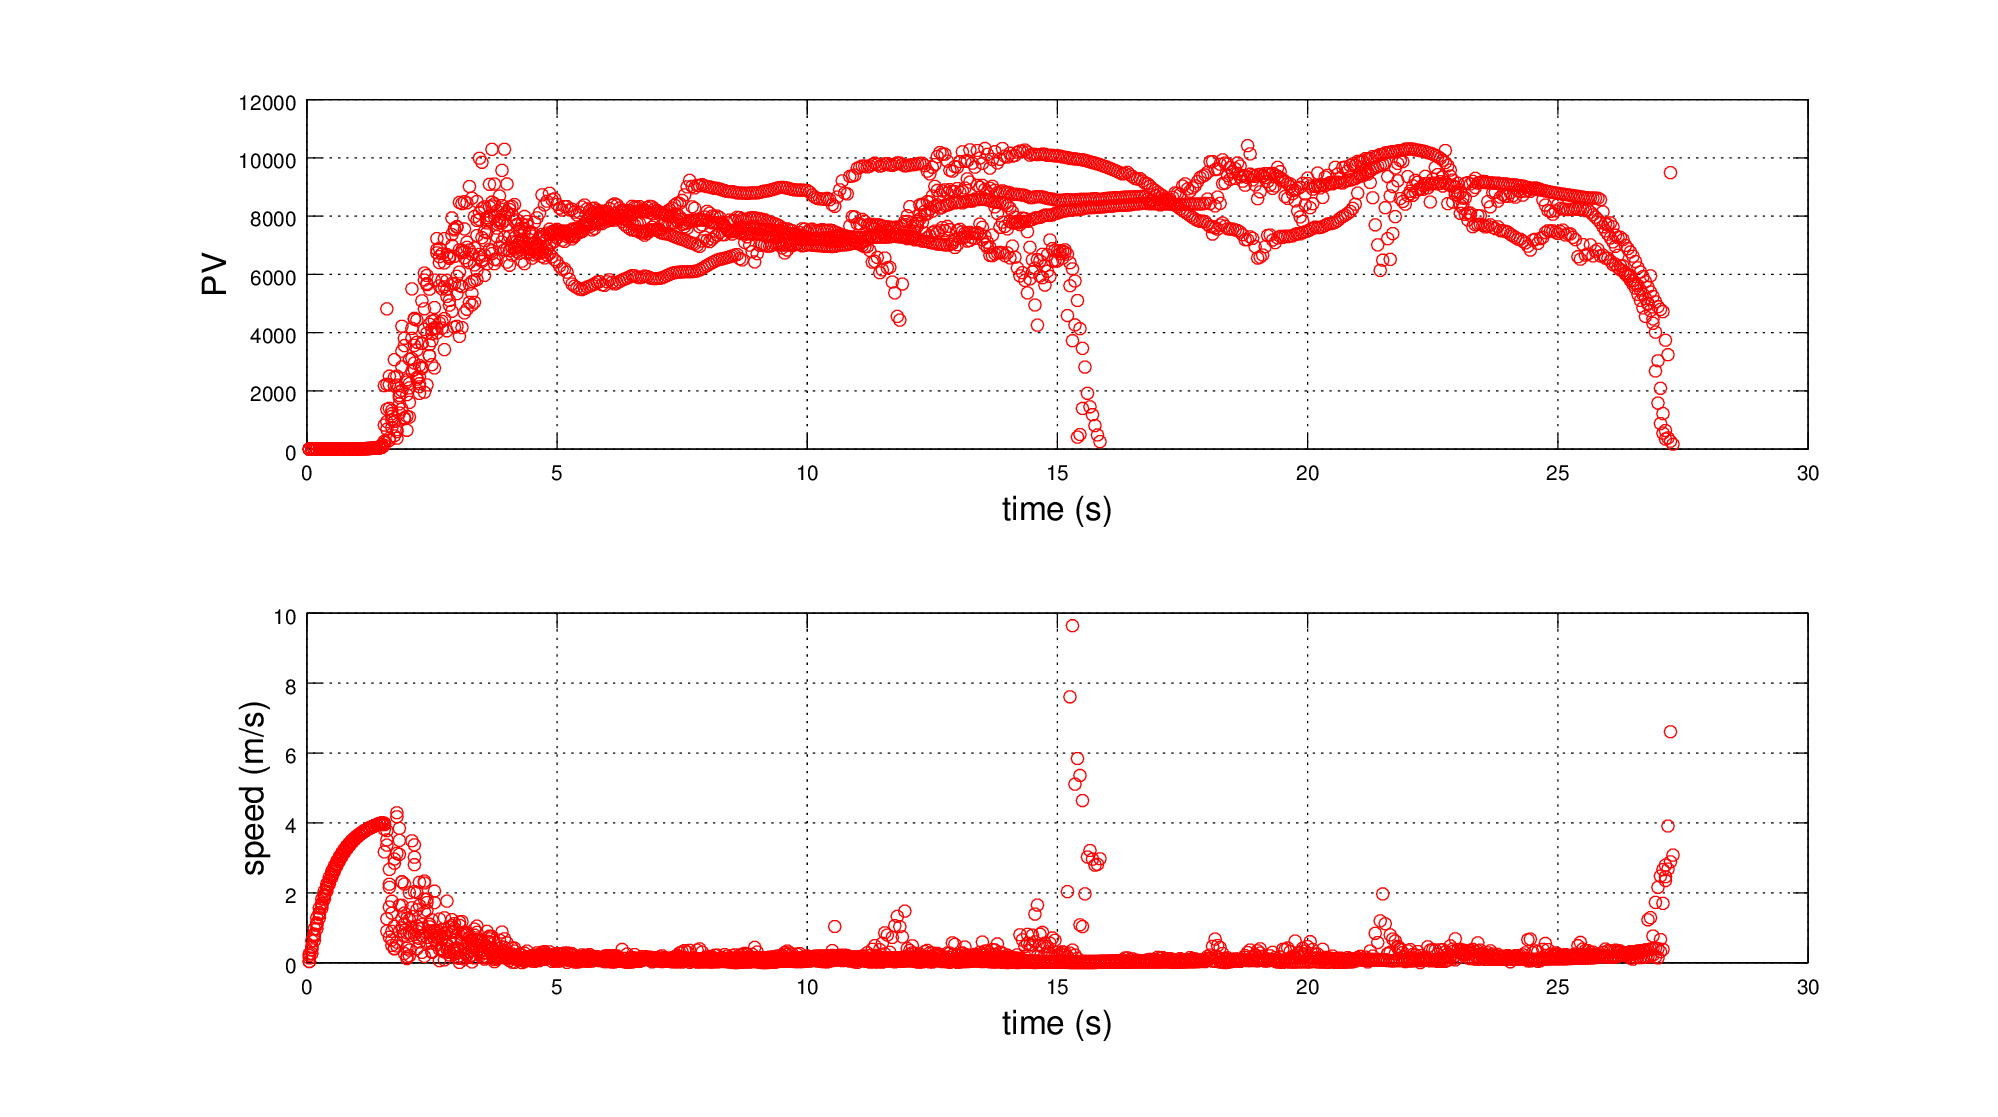
\includegraphics[height=5.5cm]{figuras/pv_vel_t_100_1_2.png}
    \caption[width=5cm]{Gráfico de velocidad(inferior) y presión(superior) en función del tiempo para un individuo ubicado inicialmente en $x=10$~m e $y=10$~m.  La salida está centrada en la posición $x=20$~m e $y=10$~m y tiene ancho $L=1,2$~m. El recinto es de $20\times 20$~(m) con 225 individuos. La gráfica corresponde a cinco iteraciones diferentes (variando la velocidad incial). La velocidad deseada del individuo fue de $v_d=4$~m/s.}
    \label{sintesis}
\end{figure}



\section{Dos puertas}

\subsection{Faster is slower}

\subsection{Tiempo de evacuación}

\begin{figure}[H]
    \centering
    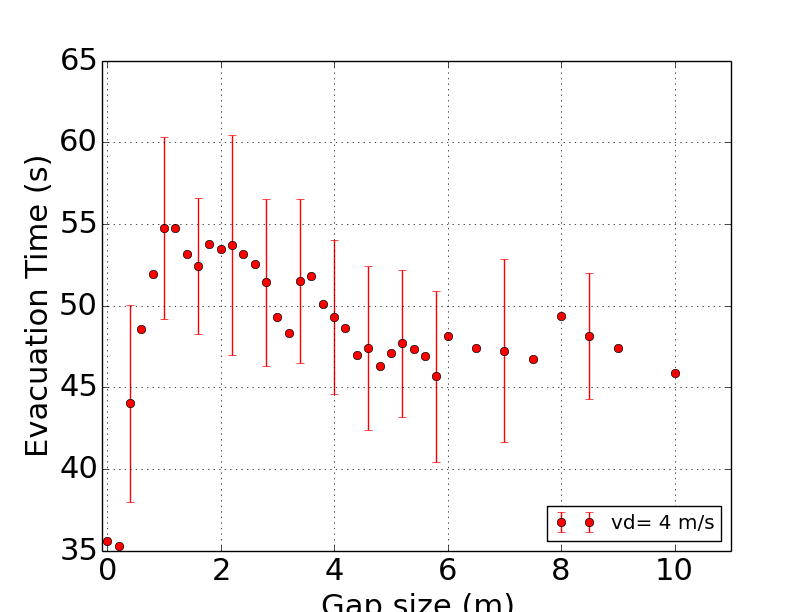
\includegraphics[height=5.5cm]{figuras/gap_vste_225p.png}
    \caption[width=5cm]{Gráfico de tiempo de evacuación en función del gap. El recinto es de $20\times 20$~(m) con 225 individuos y dos puertas, cada una tiene un ancho de $L=1,2$~m. La gráfica corresponde al promedio de treinta iteraciones. La velocidad deseada del individuo fue de $v_d=4$~m/s. Cada simulación termina cuando evacúan 160 individuos.}
    \label{sintesis}
\end{figure}

\begin{figure}[H]
    \centering
    \includegraphics[height=5.5cm]{figuras/gap_vsten.png}
    \caption[width=5cm]{Gráfico de tiempo de evacuación en función del gap para recintos de $20\times 20$~(m), $30\times 30$~(m) y $40\times 40$~(m) con 225, 580 y 961 individuos respectivamente. Todos los recintos tienen dos puertas, cada una de ancho $L=1,2$~m. Las gráficas corresponden al promedio de treinta iteraciones. Para todos los casos, la velocidad deseada del individuo fue de $v_d=4$~m/s. Cada simulación termina cuando evacúan 160, 529 y 961 individuos respectivamente.}
    \label{sintesis}
\end{figure}

\begin{figure}[H]
    \centering
    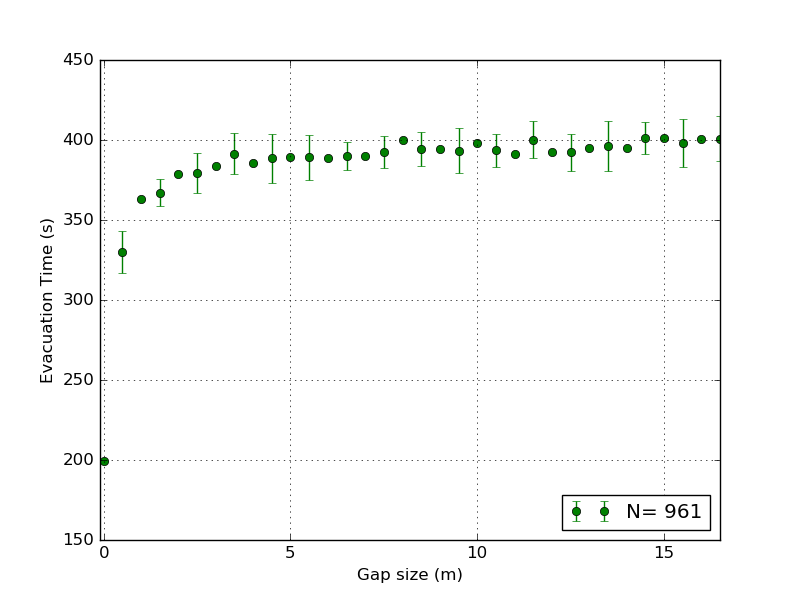
\includegraphics[height=5.5cm]{figuras/gap_vste_v4_961p.png}
    \caption[width=5cm]{Gráfico de tiempo de evacuación en función del gap. El recinto es de $40\times 40$~(m) con 961 individuos y dos puertas, cada una tiene un ancho de $L=1,2$~m. La gráfica corresponde al promedio de treinta iteraciones. La velocidad deseada del individuo fue de $v_d=4$~m/s. Cada simulación termina cuando evacúan 864 individuos.}
    \label{sintesis}
\end{figure}

\begin{figure}[H]
    \centering
    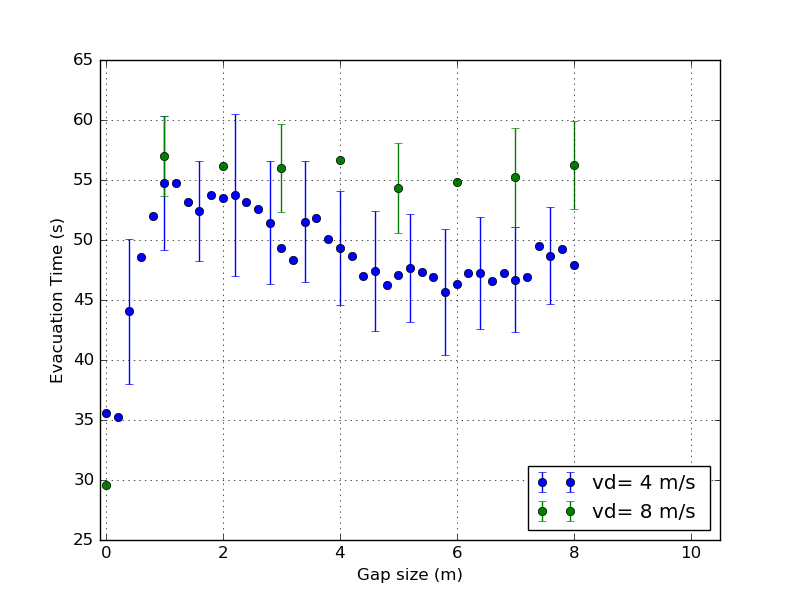
\includegraphics[height=5.5cm]{figuras/gap_vste_v4_v8.png}
    \caption[width=5cm]{Gráfico de tiempo de evacuación en función del gap. El recinto es de $20\times 20$~(m) con 225 individuos y dos puertas, cada una tiene un ancho de $L=1,2$~m. La gráfica corresponde al promedio de treinta iteraciones. Las velocidades de deseo de los individuos es de $v_d=4$~m/s y $v_d=8$~m/s. Cada simulación termina cuando evacúan 160 individuos.}
    \label{sintesis}
\end{figure}




\subsection{Blocking clusters}

\begin{figure}[H]
    \centering
    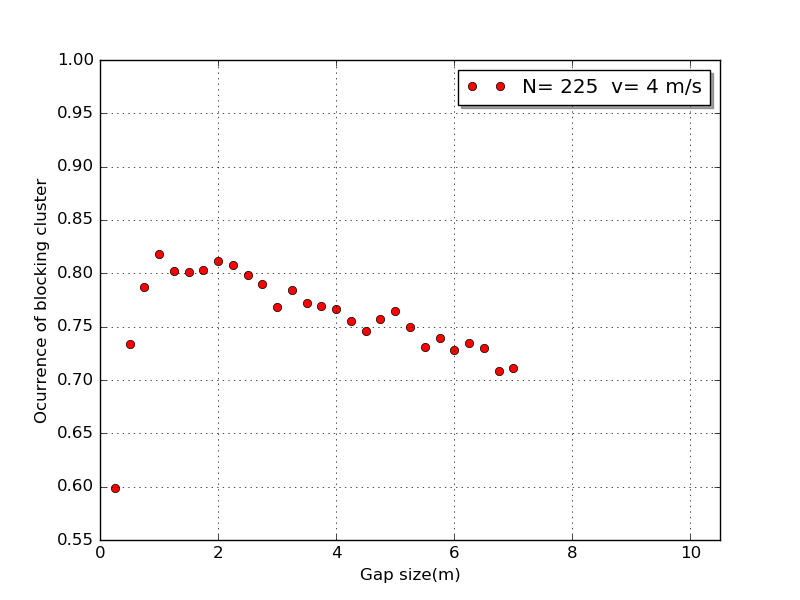
\includegraphics[height=5.5cm]{figuras/proba_vsgap_small_225p_v4.png}
    \caption[width=5cm]{Probabilidad de formar small blocking clusters (bloqueos de una sola puerta) en función del gap. El recinto es de $20\times 20$~(m) con 225 individuos y dos puertas, cada una tiene un ancho de $L=1,2$~m. La gráfica corresponde al promedio de treinta iteraciones. La velocidad de deseo es de $v_d=4$~m/s. Cada simulación termina cuando evacúan 160 individuos.}
    \label{sintesis}
\end{figure}

\begin{figure}[H]
    \centering
    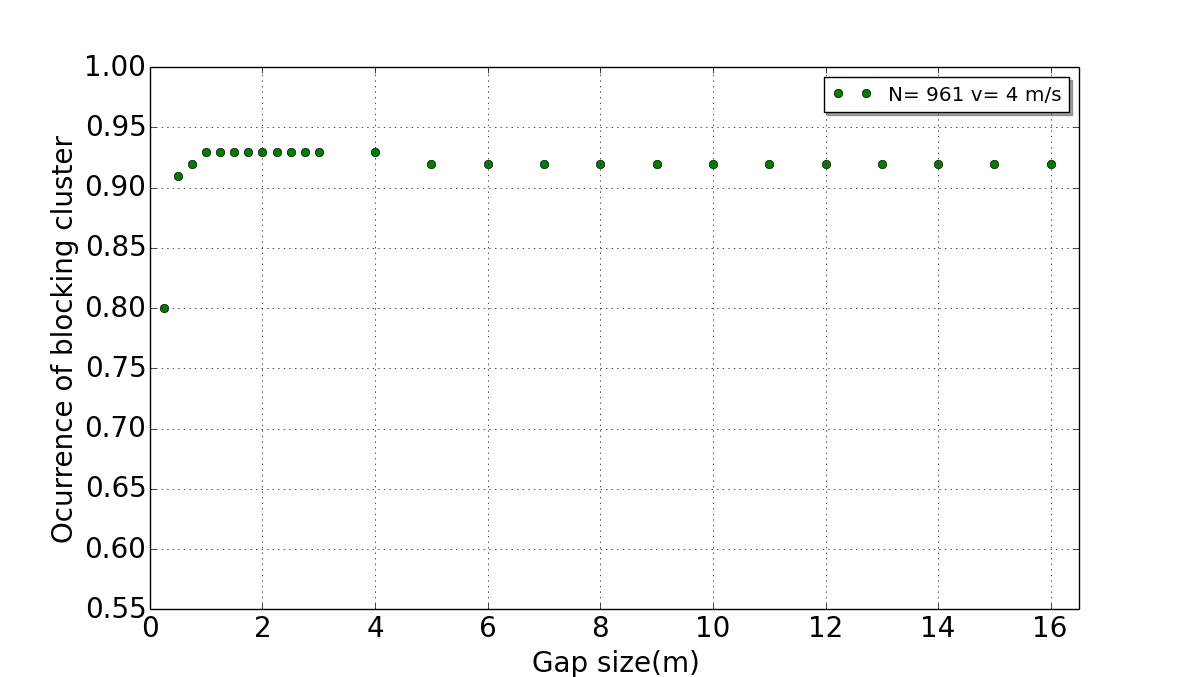
\includegraphics[height=5.5cm]{figuras/proba_vsgap_small_961p_v4.png}
    \caption[width=5cm]{Probabilidad de formar small blocking clusters (bloqueos de una sola puerta) en función del gap. El recinto es de $40\times 40$~(m) con 961 individuos y dos puertas, cada una tiene un ancho de $L=1,2$~m. La gráfica corresponde al promedio de treinta iteraciones diferentes. La velocidad de deseo es de $v_d=4$~m/s. Cada simulación termina cuando evacúan 864 individuos.}
    \label{sintesis}
\end{figure}

\begin{figure}[H]
    \centering
    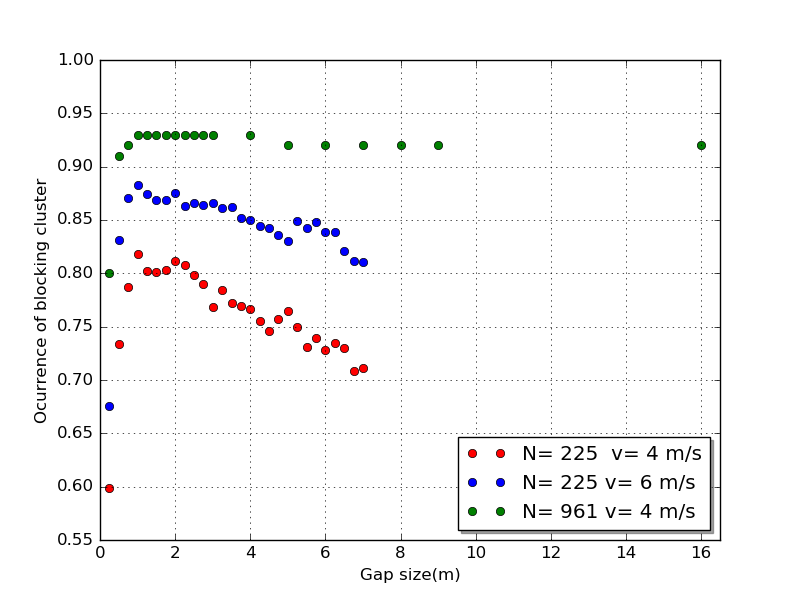
\includegraphics[height=5.5cm]{figuras/proba_vsgap_small_all.png}
    \caption[width=5cm]{Probabilidad de formar small blocking clusters (bloqueos de una sola puerta) en función del gap, para un recinto $20\times 20$~(m) con 225 individuos a $v_d=4$~m/s y $v_d=6$~m/s. Lo mismo para un recinto de $40\times 40$~(m) con 961 individuos a $v_d=4$~m/s. Ambos recintos poseén dos puertas, cada una tiene un ancho de $L=1,2$~m. Las gráficas corresponden al promedio de treinta iteraciones diferentes. Las simulación terminan cuando evacúan 160 individuos y 864 respectivamente.}
    \label{sintesis}
\end{figure}

\begin{figure}[H]
    \centering
    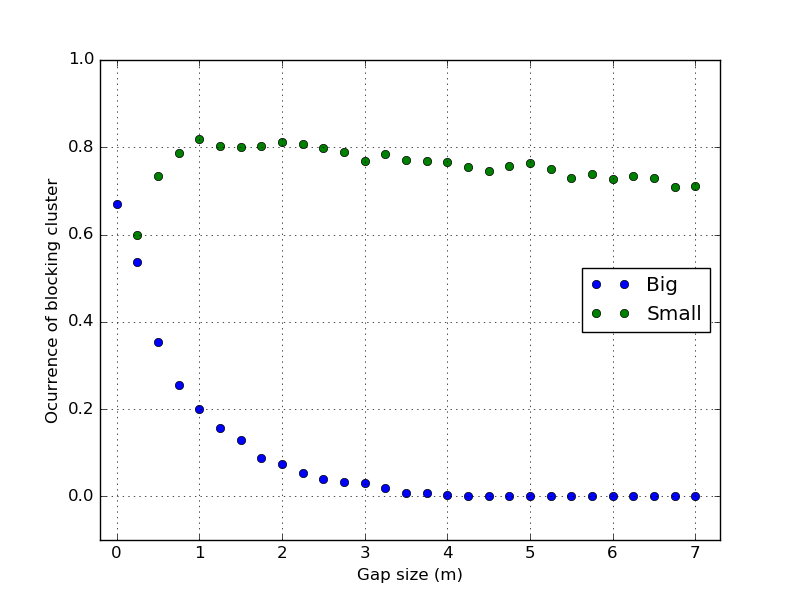
\includegraphics[height=5.5cm]{figuras/proba_vsgap_v4_big_small.png}
    \caption[width=5cm]{Probabilidad de formar big y small blocking clusters (bloqueos de dos y una puerta respectivamente) en función del gap. El recinto es de $20\times 20$~(m) con 225 individuos y dos puertas, cada una tiene un ancho de $L=1,2$~m. Las gráficas corresponden al promedio de treinta iteraciones diferentes. La velocidad de deseo es de $v_d=4$~m/s. Cada simulación termina cuando evacúan 160 individuos.}
    \label{sintesis}
\end{figure}



\subsection{Presión}

\begin{figure}[H]
    \centering
    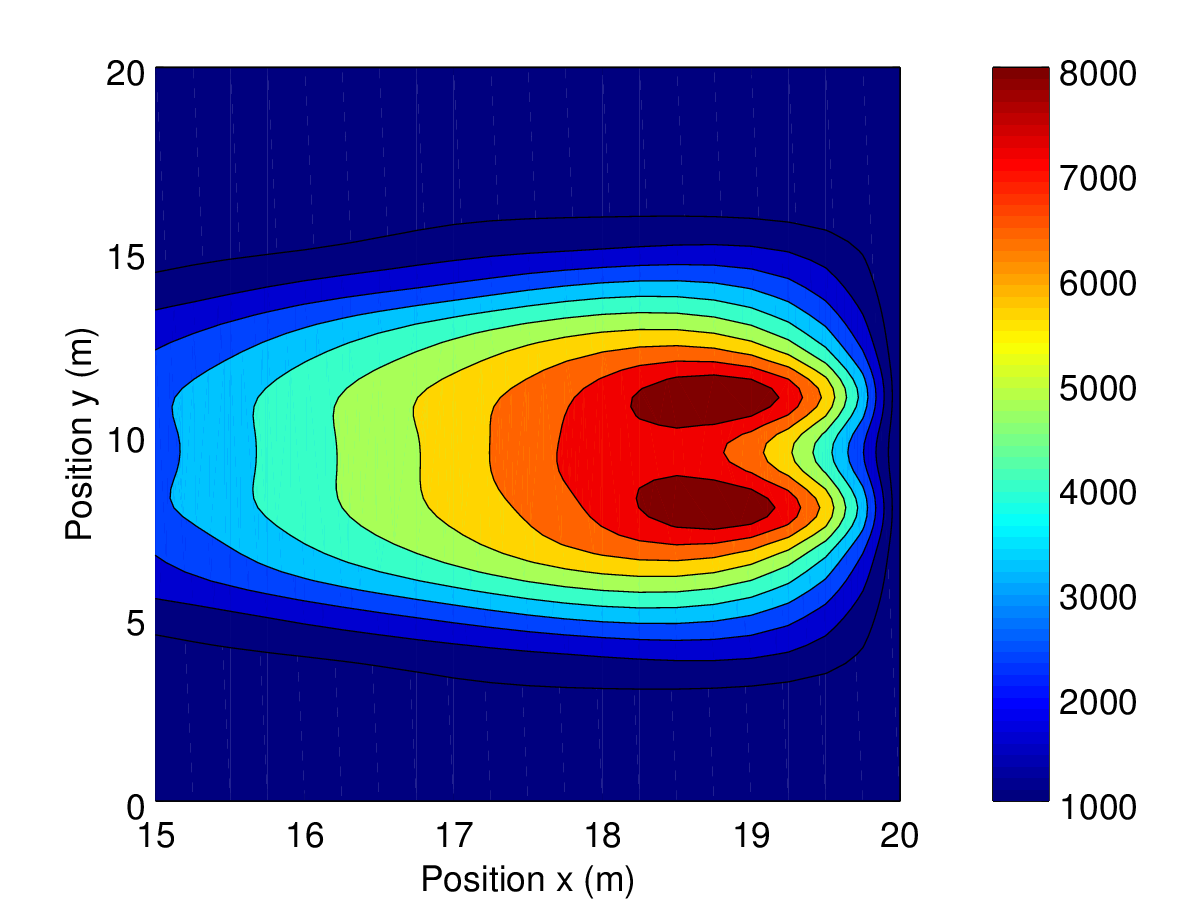
\includegraphics[height=5.5cm]{figuras/press_225p_v4_g0.png}
    \caption[width=5cm]{Isobaras cercanas a la puerta; la escala a la derecha está expresada en [PV]=N.m. La salida está centrada en la posición $x=20$~m e $y=10$~m, son dos puertas de ancho $L=1,2$~m con $g=0$~m. El recinto es de $20\times 20$~(m) con 225 individuos. La gráfica corresponde a valores medios a lo largo de 30 procesos de evacuación. Se usó un grillado de 1m$^2$ para promediar el campo de presiones (PV). La velocidad deseada de los individuos fue de $v_d=4$~m/s.}
    \label{presion_225p_g0}
\end{figure}

\begin{figure}[H]
    \centering
    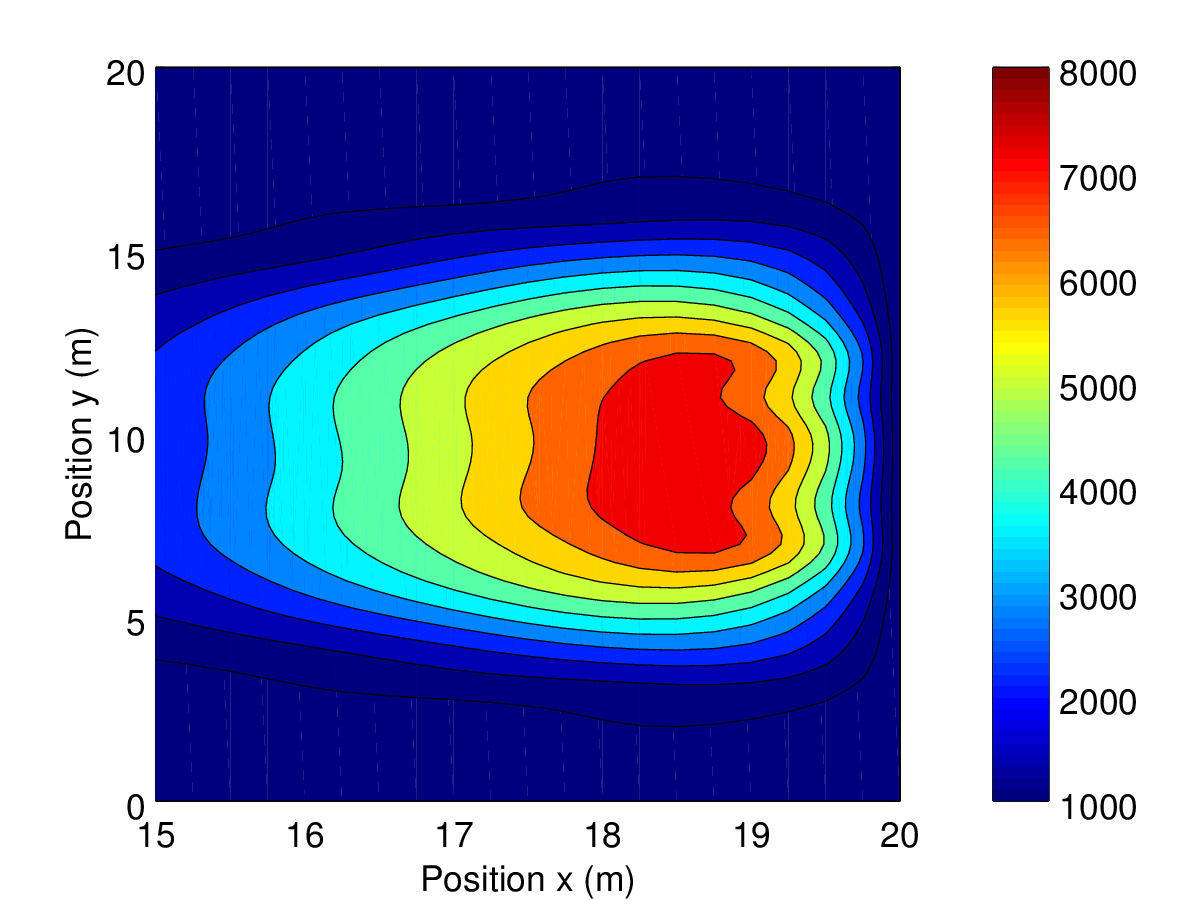
\includegraphics[height=5.5cm]{figuras/press_225p_v4_g1_5.png}
    \caption[width=5cm]{Isobaras cercanas a la puerta; la escala a la derecha está expresada en [PV]=N.m. La salida consta de dos puertas de ancho $L=1,2$~m separadas entre si por una distancia de $g=1,5$~m, centrdas en $x=20$~m e $y=11,35$~m y $x=20$~m e $y=8,65$~m . El recinto es de $20\times 20$~(m) con 225 individuos. La gráfica corresponde a valores medios a lo largo de 30 procesos de evacuación. Se usó un grillado de 1m$^2$ para promediar el campo de presiones (PV). La velocidad deseada de los individuos fue de $v_d=4$~m/s.}
    \label{presion_225p_g1_5}
\end{figure}

\begin{figure}[H]
    \centering
    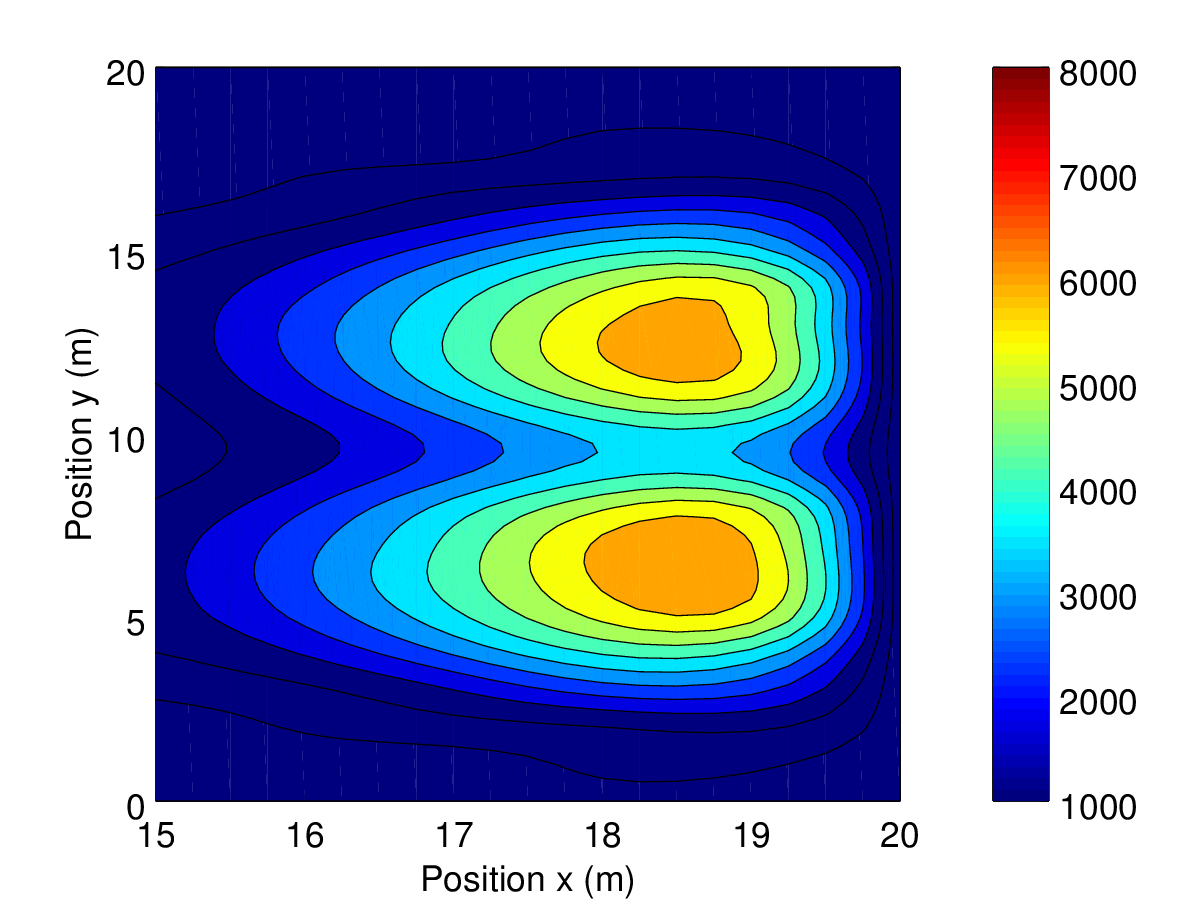
\includegraphics[height=5.5cm]{figuras/press_225p_v4_g5.png}			\caption[width=5cm]{Isobaras cercanas a la puerta; la escala a la derecha está expresada en [PV]=N.m. La salida consta de dos puertas de ancho $L=1,2$~m separadas entre si por una distancia de $g=1,5$~m, centrdas en $x=20$~m e $y=12,5$~m y $x=20$~m e $y=7,5$~m. El recinto es de $20\times 20$~(m) con 225 individuos. La gráfica corresponde a valores medios a lo largo de 30 procesos de evacuación. Se usó un grillado de 1m$^2$ para promediar el campo de presiones (PV). La velocidad deseada de los individuos fue de $v_d=4$~m/s.}
    \label{presion_225p_g5}
\end{figure}




%\subsection{Velocidad}
\subsection{Comportamiento asintótico}




